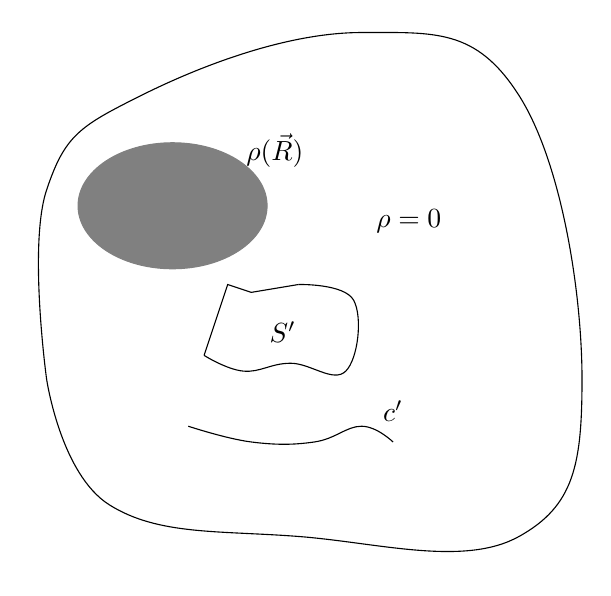
\begin{tikzpicture}

\draw  plot[smooth, tension=.7] coordinates {(-2.4,-0.4) (-1.6,-2) (0.8,-2.4) (3.6,-2.4) (4.4,-0.4) (3.6,3.2) (1.6,4) (-1.2,3.2) (-2.4,2) (-2.4,-0.4)};
\node (p1) at (-0.8,1.8) {};
\draw  [fill, gray] (p1) ellipse (1.2 and 0.8);
\draw  plot[smooth, tension=.7] coordinates {(-0.6,-1) (0.2,-1.2) (1,-1.2) (1.6,-1) (2,-1.2)} node [above=4] {$c'$};
\draw  plot[smooth, tension=.7] coordinates {(-0.4,-0.1) (0.1,-0.3) (0.7,-0.2) (1.4,-0.3) (1.5,0.6) (0.8,0.8)};
\draw (0.8,0.8) -- (0.2,0.7) -- (-0.1,0.8) -- (-0.4,-0.1);
\node at (0.6,0.2) {$S'$};
\node at (2.2,1.6) {$\rho=0$};
\node at (0.5,2.5) {$\rho(\vec{R})$};
\end{tikzpicture}